\chapter{Ultrasound Applikation}
In diesen Kapitel werden Informationen zur Applikation und deren Umsetzung vermittelt. Dabei werden der Aufbau einer Sonde und deren Anpassung an die Dopplerapplikation, die aktuelle Umsetzung der Datenerfassung und -verarbeitung, sowie die mögliche Datenausgabe durch Bilderzeugung beschrieben.
\section{Transducer}
Um die elektrische Energie in mechanische Energie und umgekehrt zu wandeln wird ein Transducer benötigt, welcher gleichzeitig das Kernstück der Ultraschallsonographie darstellt.
\begin{figure}[ht]
\centering
  	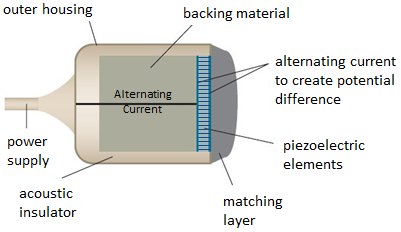
\includegraphics[width=0.65\textwidth]{Ultrasound/Transducer-Workings} 
  \caption[Transducer Aufbau]{Transducer Aufbau \cite{agnieszka}}
  \label{fig:transducher}
\end{figure}\\
Dieser besteht wie in \autoref{fig:transducher} gezeigt aus einen Piezoelement mit der dazugehörigen matching-Schicht für die verbesserte Fokussierung. Da die longitudinal Wellen auf beiden Seiten eines Piezoelementes entstehen, müssen die Wellen auf der Rückseite der Sonde absorbiert werden um Reflektionen zu vermeiden. Dies geschieht durch einen akustischen Absorber und einen Dämpfungsblock. Zudem muss die Sonde vor \ac{emi} Störungen geschützt werden, da das Piezoelement auf einstrahlende Frequenzen reagieren kann. Dies geschieht durch ein geschirmtes Metallgehäuse welches an der Messstation geerdet ist und somit die Störungen ableiten kann.\\
Für die Bestimmung der Arbeitsfrequenz $f_0$ kann grundlegend gesagt werden, dass die genierten Frequenzen umgekehrt proportional zur Dicke des Piezoelementes $l_{piezo}$ sind. Um möglichst viel Energie effektiv umwandeln zu können, wird das Piezoelement bei möglichst geringer Impedanz betrieben. Dabei sollte die Phasenverschiebung 0$^\circ$ betragen, um keine Blindleistung zu generieren. Dabei ist zu beachten, dass das Element schnellstmöglich ein- und ausschwingen soll, wodurch es am besten in Resonanz betrieben wird. Ein Piezoelement vibriert in Resonanz, wenn die Dicke $l_{piezo}$ gleich $1/2\lambda$ ist\cite[S. 35]{brucher_ultra}, wodurch sich folgende Formel für die Bestimmung der Arbeitsfrequenz $f_0$ eines Piezoelementes aufstellen lässt.
\begin{align}
l_{piezo}&=\frac{1}{2}\lambda =\frac{1}{2} \frac{c}{f_0}\\
f_0&=\frac{c}{2\cdot l_{piezo}}
\end{align}
\section{Kristall-Impedanz-Matching}
Nachdem die zu emittierende Frequenz und somit die Kristalldicke definiert wurde, muss durch das Verhalten des ausgewählten Kristalls eine Impedanzanpassung durchgeführt werden, da dieser eine Serien- und eine Parallelresonanz besitzt. Dieser Schritt ist nötig, da das Schleifen der Kristalle Fertigungstoleranzen unterliegt, und somit Kristalle nicht genau auf die zu emittierende Frequenz geschliffen werden können. Als Beispiel wurde ein idealer 2 \ac{mhz} Kristall in \autoref{fig:piezo} dargestellt, wobei die Resonanzen um \ac{ca} 5 \ac{khz} nach oben verschoben sind.
\begin{figure}[h!]
	\centering
        \begin{subfigure}[t]{0.48\textwidth}
                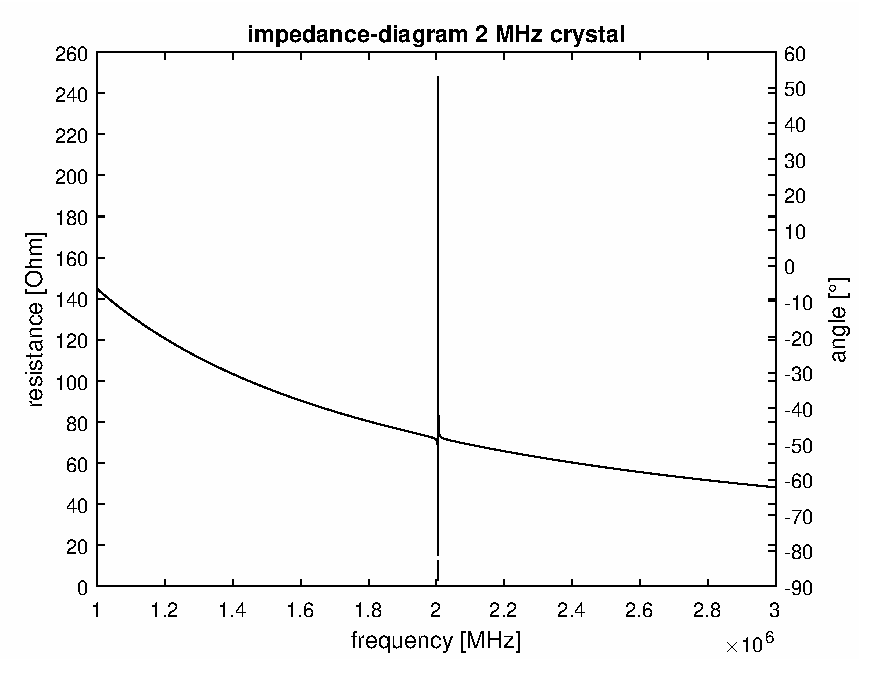
\includegraphics[width=1\textwidth]{images/Ultrasound/zoom_out.eps}
	    		\caption{Impedanz-Diagramm}
	    		\label{fig:imp_2mhz_without}
        \end{subfigure}
        ~ %add desired spacing between images, e. g. ~, \quad, \qquad, \hfill etc.
          %(or a blank line to force the subfigure onto a new line)
        \begin{subfigure}[t]{0.48\textwidth}
        	 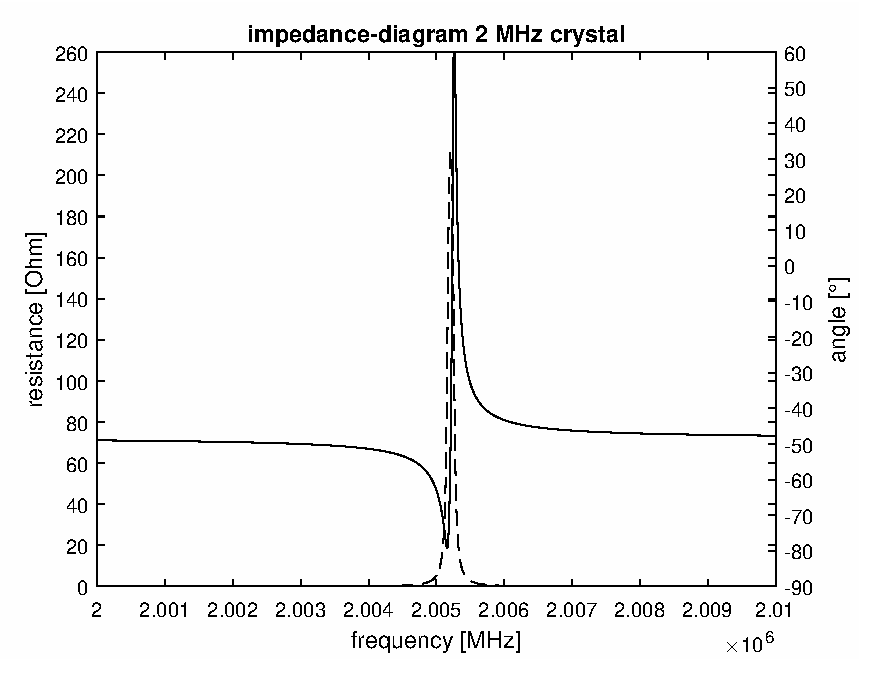
\includegraphics[width=1\textwidth]{images/Ultrasound/zoom_in.eps}
	    		\caption{Impedanz-Diagramm - Zoom}
	    		\label{fig:imp_2mhz_with}
        \end{subfigure}
	\caption{2 \acs{mhz} Piezokristall ohne Anpassung}
	\label{fig:imp_2mhz_without}
\end{figure}\\
Um die Effektivität, \ac{resp} die zu emittierende Energie, zu steigern, wird eine Leistungsanpassung benötigt. Hierzu wird das elektrische \ac{esb} eines Piezokristalls herangezogen, welches durch die Parameter in \autoref{tab:var_esb} definiert und in \autoref{fig:esb_without} visualisiert ist.
\begin{figure}[h!]
	\centering
	\begin{subfigure}[b]{0.42\textwidth}
		\centering
  		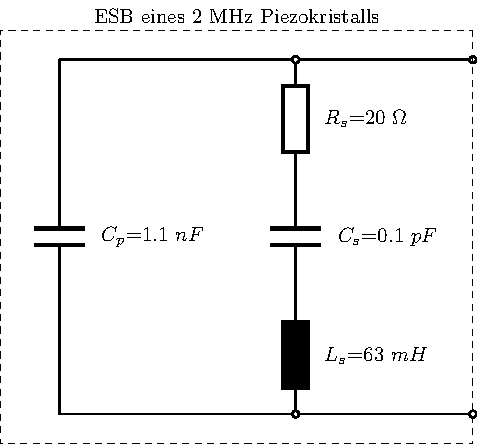
\includegraphics[width=0.95\textwidth]{images/Ultrasound/ESB}
  		\caption{ohne Anpassung}
  		\label{fig:esb_without}
  	\end{subfigure}
  	\hfill
  	\begin{subfigure}[b]{0.56\textwidth}
	  	\centering
		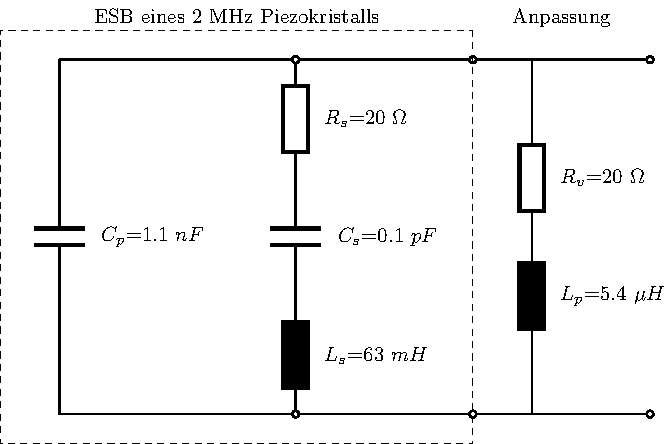
\includegraphics[width=1\textwidth]{images/Ultrasound/ESB_with_inductance}
  		\caption{Anpassung mit Leitungsverlust und Induktivität}
  		\label{fig:esb_with}
  	\end{subfigure}
  	\caption{\acs{esb} eines 2 \acs{mhz} Piezokristalls}
  	\label{fig:piezo}
\end{figure}\\
Eine Leistungsanpassung erfolgt in \autoref{fig:esb_with} wobei mit Verlusten durch die Leitungslänge zu rechnen ist. Für die Parallelabstimmung des Kristalls wird die parallele Induktivität $L_{p}$ bestimmt, indem die \autoref{eq:imp_lp} für die Berechnung herangezogen wird.
\begin{equation}
L_{p}=\dfrac{1}{\omega_s^2\cdot C_p}\ mit\ \omega_s=2\pi f_s\label{eq:imp_lp}
\end{equation}
Dabei ergibt sich bei einer geforderten Nutzfrequenz $f_s$ von 2 \ac{mhz} eine parallele Induktivität $L_p$ von rund 6,3 $\mu$H. Da 6,3 $\mu$H Induktivitäten nicht bezogen werden können, beziehen sich nachfolgende Betrachtungen auf 2 beziehbare 2,7 $\mu$H Induktivitäten in Serie.
\begin{figure}[h!]
	\centering
         ~ %add desired spacing between images, e. g. ~, \quad, \qquad, \hfill etc.
          %(or a blank line to force the subfigure onto a new line)
        \begin{subfigure}[t]{0.48\textwidth}
        	 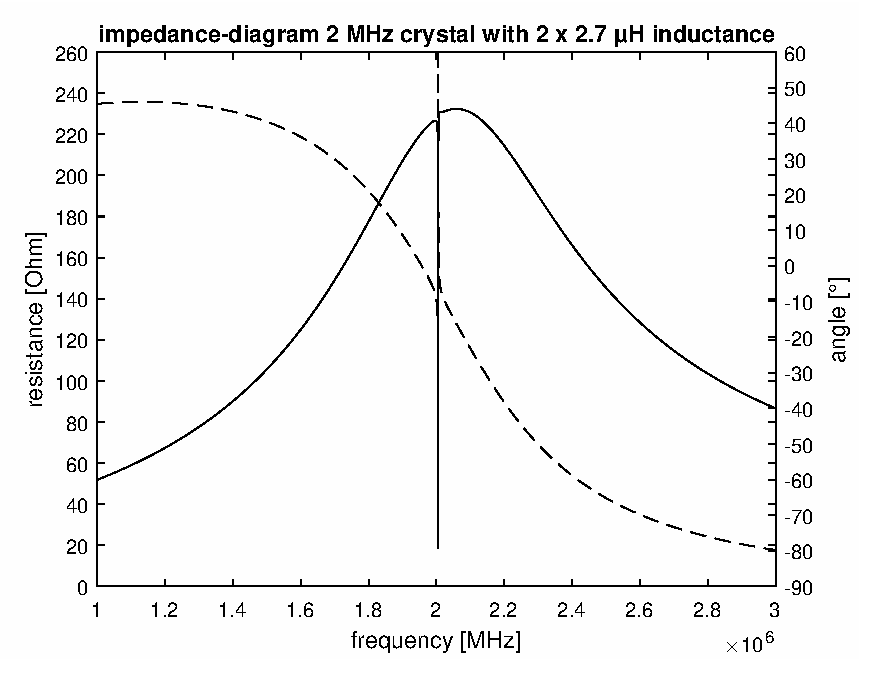
\includegraphics[width=1\textwidth]{images/Ultrasound/zoom_out_with.eps}
	    		\caption{Impedanz-Diagramm}
	    		\label{fig:imp_2mhz_with}
        \end{subfigure}	
         ~ %add desired spacing between images, e. g. ~, \quad, \qquad, \hfill etc.
          %(or a blank line to force the subfigure onto a new line)
        \begin{subfigure}[t]{0.48\textwidth}
        	 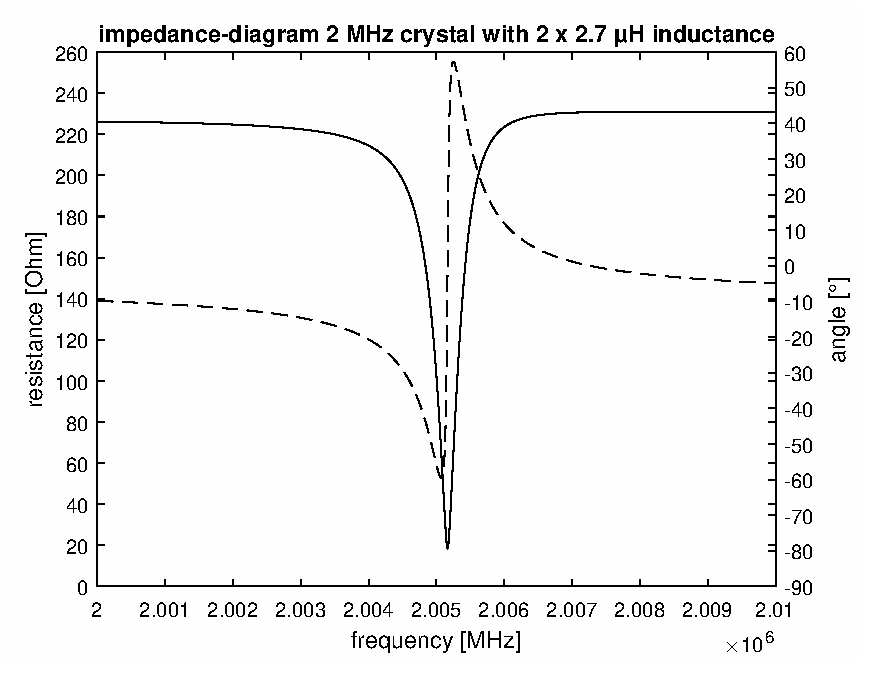
\includegraphics[width=1\textwidth]{images/Ultrasound/zoom_in_with.eps}
	    		\caption{Impedanz-Diagramm - Zoom}
	    		\label{fig:imp_2mhz_with}
        \end{subfigure}	
	\caption{2 \acs{mhz} Piezokristall mit Anpassung}
	\label{fig:imp_2mhz_with}
\end{figure}\\
Vergleicht man \autoref{fig:imp_2mhz_without} mit \autoref{fig:imp_2mhz_with} ist ersichtlich, dass die Resonanzen weiter auseinander liegen. Zudem liegt die Phase bei der Nutzfrequenz nicht mehr zwischen -80$^\circ$ und 30$^\circ$ sondern zwischen $\pm$55$^\circ$. Das wichtigste Argument der durchgeführten Anpassung ist jedoch ersichtlich, wenn man die Breitbandigkeit des Kristalls betrachtet. Durch das Kristall-Impedanz-Matching wird die Breitbandigkeit des Kristalls gesteigert, was die für die Doppler-Schiebefrequenzen von $\pm$12 \ac{khz} um die Trägerfrequenz notwendig ist. Somit werden höhere Schiebefrequenzen weniger gedämpft, die bei erhöhten Fließgeschwindigkeiten in Arterien durch das Strömungsprofil auftreten.\\
Diese Methode steigert durch die reduzierte Amplitudendämpfung der reflektierten dynamischen Echos die Erkennung von schnell wandernden Embolien.
\section{Quadraturdemodulation}\label{sec:demodulate}
\begin{figure}[h!t]
\centering
\begin{tikzpicture}
	\matrix (m0) [row sep=2.5mm, column sep=12mm]
	{	%--------------------------------------------------------------------
		\node[coordinate]                  (m00) {};   		  &
		\node[coordinate]                  (m01) {};   		  &
		\node[dspmixer, pin={[pin edge={to-,very thick,black}]below:$cos(2\pi f_0)$}]                    (m02) {};   		  &
		\node[dspsquare]                   (m03) {LPF};   	  &
		\node[dspnodeopen,dsp/label=below] (m0X) {$I(t)$};	  \\				%--------------------------------------------------------------------
		\node[dspnodeopen,dsp/label=above] (m10) {$f_{RF}(t)$};    &
		\node[dspnodefull]                 (m11) {};          &
		\node[coordinate]                  (m12) {};          &
		\node[coordinate]                  (m13) {};          &
		\node[coordinate]                  (m1X) {};          \\		%--------------------------------------------------------------------
		\\		%--------------------------------------------------------------------
		\node[coordinate]                  (m20) {};          &
		\node[coordinate]                  (m21) {};          &
		\node[dspmixer, pin={[pin edge={to-,very thick,black}]below:$sin(2\pi f_0)$}]                    (m22) {};   		  &
		\node[dspsquare]                   (m23) {LPF};		  &
		\node[dspnodeopen,dsp/label=below] (m2X) {$Q(t)$};    \\		%--------------------------------------------------------------------		%--------------------------------------------------------------------
		\node[coordinate] (m30) {}; &
		\node[coordinate] (m31) {}; &
		\node[coordinate] (m32) {}; &
		\node[coordinate] (m33) {}; &
		\node[coordinate] (m3X) {};    \\		%--------------------------------------------------------------------
	};	
	\begin{scope}[start chain]
		\chainin (m10);
		\chainin (m11) [join=by dspconn];
		\chainin (m01) [join=by dspline];
		\chainin (m21) [join=by dspline];
	\end{scope}
	%\draw[dspconn]  (m12) --  (m02);	
	%\draw[dspconn]  (m32) -- node[below] {$sin(2\pi f_0)$} (m22);	
			
	\foreach \i [evaluate = \i as \j using int(\i+1)] in {1,..., 2}
	{
		\draw[dspconn] (m0\i) -- (m0\j);
		\draw[dspconn] (m2\i) -- (m2\j);
	}
	\draw[dspflow] (m03) -- (m0X);
	\draw[dspflow] (m23) -- (m2X);
\end{tikzpicture}
\caption{Blockdiagramm Quadraturdemodulation und Tiefpass}
\label{fig:demo}
\end{figure}
Die Quadraturdemodulation ist eine Möglichkeit, Hochfrequente Eingangssignale in den Niederfrequenzbereich umzuwandeln. Dabei wird das Eingangssignal \(f_{RF}(t)\) mit der Trägerfrequenz \(f_0\) multipliziert \ac{bzw} gemischt, wodurch ein Frequenzgemisch aus Summe \(f_0+f_{RF}\) und Differenz \(f_0-f_{RF}\) entsteht. Der allgemeine Mischprozess ist dabei durch die Hochfrequenz \(f_{RF}\), den lokalen Oszillator \(f_{0}\) und die Zwischenfrequenz \(f_{IF}\) definiert, wobei die Frequenz am Ausgang durch \autoref{eq:mischer} definiert ist.\cite[S. 2 f.]{mischer} 
\begin{equation}
f_{IF}=\vert f_{RF}\pm f_{0}\vert\label{eq:mischer}
\end{equation}
Um die Summenfrequenz zu unterdrücken, wird für die Quadraturdemodulation ein Tiefpassfilter verwendet, da die niederfrequenten Doppler-Schiebefrequenzen von wenigen \ac{khz} genutzt werden sollen. Dabei werden die Summenfrequenzen der Multiplikation eliminiert. Diese Technik wird auch als moving average Filter bezeichnet.\\
Um die Differenzfrequenz (oberes Seitenband) von der sogenannten Spiegelfrequenz\cite[S. 3]{mischer}(unteres Seitenband) und somit die Richtung bewegter Objekte, welche in dieser Applikation Blut und mögliche Embolien darstellen, zu unterscheiden, wird die Phaseninformation des Signals \(f_{RF}\) benötigt. Dabei wird die Oszillatorfrequenz \(f_{0}\) um 90$^\circ$ verschoben und mit dem Eingangssignal \(f_{RF}\) multipliziert, wodurch das sogenannte quadrature-Signal $Q(t)$ erzeugt wird. Das inphase-Signal $I(t)$ entsteht durch Multiplikation von der Oszillatorfrequenz \(f_{0}\) um 0$^\circ$ mit der Eingangssignal \(f_{RF}\). \\
Da diese Signale um 90$^\circ$ verschoben sind, kann die Ausgangsamplitude $A(t)$ durch \autoref{eq:amplitude} berechnet werden.
\[A(t) = \sqrt{I(t)^2\cdot Q(t)^2}\]\label{eq:amplitude}
Dabei sollte beachtet werden, dass durch den nachgestellten Tiefpassfilter der I-/Q-Signale ein Quantisierungsfehler entsteht. Aus diesen Grund können nur relative Aussagen über die Amplitude des Signals gemacht werden.
\section{Implementierung}
Die Umsetzung aktueller \ac{pw}-Doppler Systeme und der Erzeugung der I/Q-Signale erfolgt durch diskrete Bauelemente und ist in \autoref{fig:analog_pwd_bloc} schematisch visualisiert. Dabei erfolgt die Ansteuerung der Peripherie wie in \autoref{fig:demodulator}. Vergleicht man das Ereignis-Zeitdiagramm von \autoref{fig:demodulator} mit dem Ereignis-Zeitdiagramm des \nameref{sec:pw} aus \autoref{sec:pw} wird ersichtlich, dass die Digitalisierung nach der Demodulierung stattfindet. Außerdem kann durch den Integrator und das Sample-and-Hold Verfahren des Tiefpassfilters nur eine \ac{roi} digitalisiert werden, wodurch ein erhöhter Hardwareaufwand für mehrere \ac{roi}s benötigten wird.
\begin{figure}[h!]
  \centering
  \begin{subfigure}[b]{1\textwidth}
	\centering
  \includegraphics[page=2,trim = 13mm 60mm 1mm 58mm, clip=true, width=\textwidth]{Ultrasound/pw_rx} 
  \caption{Block Diagramm eines analogen \ac{pw} Doppler Systems}
  \label{fig:analog_pwd_bloc}
  \end{subfigure}
  ~
  \begin{subfigure}[b]{1\textwidth}
	\centering
	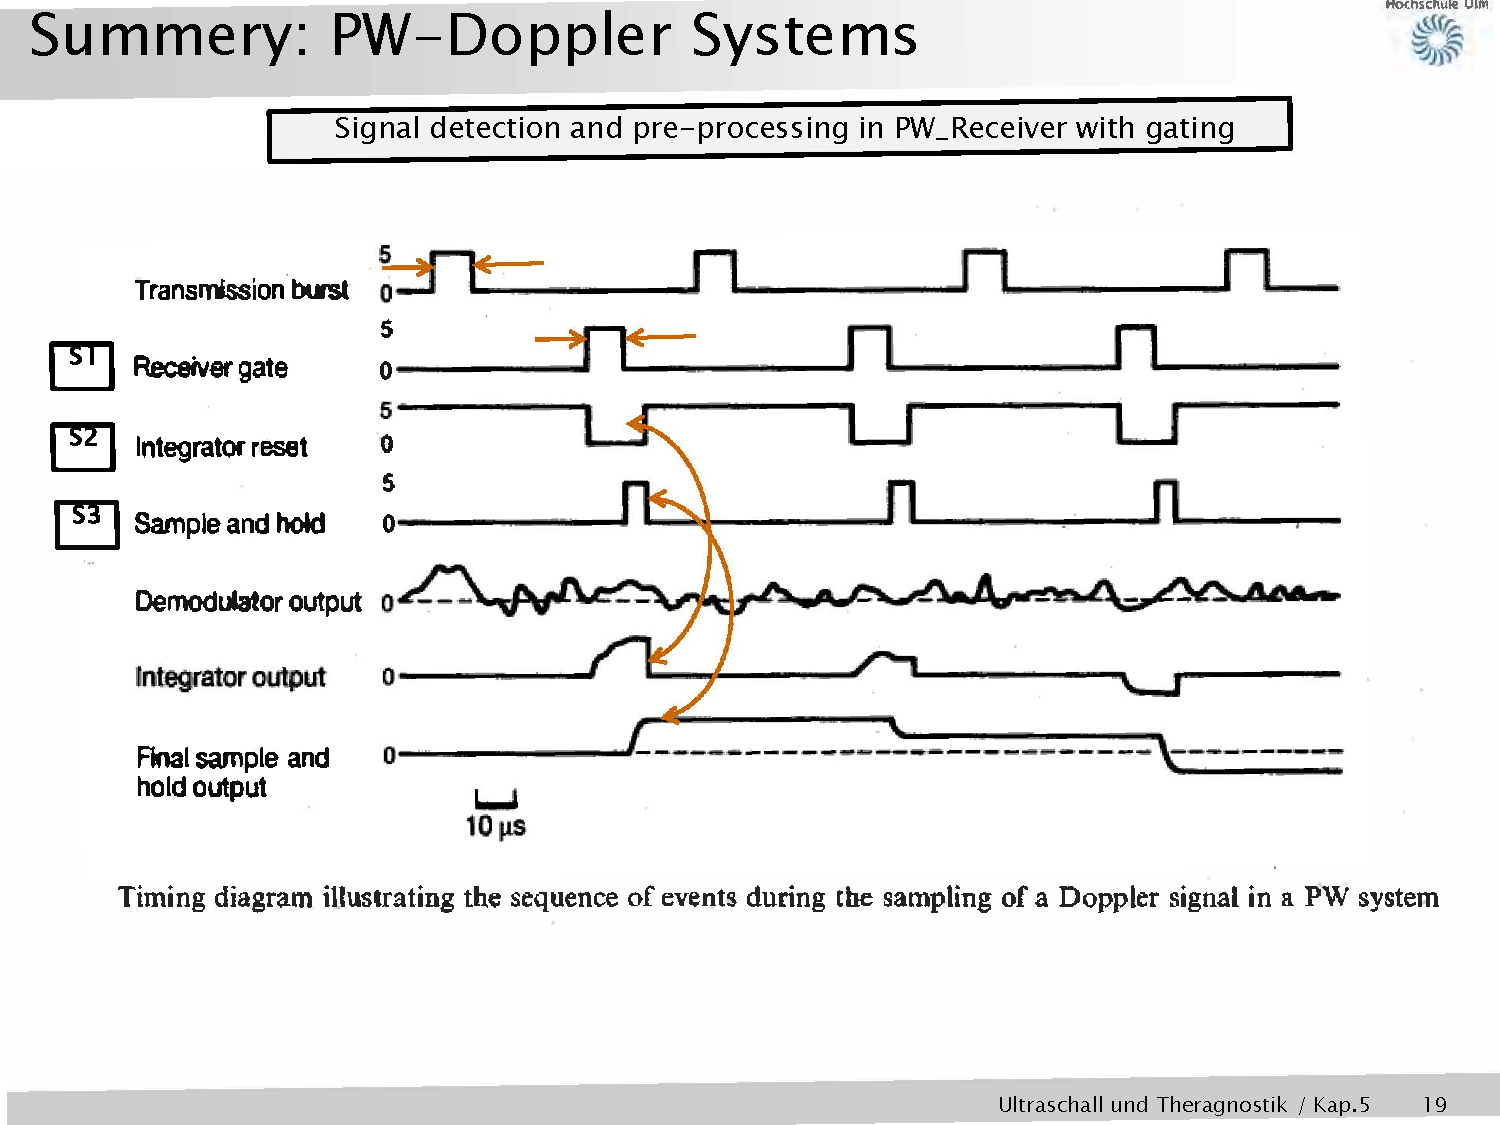
\includegraphics[page=1,trim = 23mm 48mm 27mm 42mm, clip=true, width=\textwidth]{Ultrasound/pw_rx} 
	\caption{Ereignis-Zeitdiagramm für die Verarbeitung eines analogen Demodulatorausgangs}
  \label{fig:demodulator}
  \end{subfigure}
  \caption{Block Diagramm und Ereignis-Zeitdiagramm für die Ansteuerung eines Demodulatorausgangs}
  \label{fig:analog_pwd}
\end{figure}\\
Die Digitalisierung der Daten erfolgt mit wenigen \ac{sps}, da die I/Q-Signale durch den vorgeschalteten Demodulator Phasenverschoben und auf wenige \ac{khz} gemischt werden.
\section{Auswertung der Ultraschallmessung und Bildentstehung}
\begin{figure}[h!]
  \centering
  \begin{subfigure}[b]{0.7\textwidth}
  \includegraphics[page=3,trim = 80mm 88mm 38mm 52mm, clip=true, width=\textwidth]{Ultrasound/pw_rx} 
  \caption{Hüllkurve - Amplitude der I/Q-Signale}
  \label{fig:a_mode}
\end{subfigure}
~
\begin{subfigure}[b]{0.2\textwidth}
  \centering
  \includegraphics[trim = 80mm 0mm 0mm 0mm, clip=true, height=4cm,]{Ultrasound/b-Mode}  
  	\caption{B-Mode}
  \label{fig:b_mode}
  \end{subfigure}
	\caption{A- und B-Mode}
\end{figure}
\subsection{A-Mode}\label{a-mode}
Der \glqq Amplitudenmodus\grqq{} ist die erste Darstellungsform in der Sonographie und die einfachste Umsetzung des Impuls-Echo-Prinzips. Es ist eine eindimensionale Abbildung der reflektierten Schallwellen in einem Diagramm und stellt die empfangenen Echos in Abhängigkeit von der Tiefe dar, wie in \autoref{fig:a_mode} zu sehen ist.\\
Für die Berechnung der Magnitude $B_a(t)$ werden die I/Q-Signale $I(t),Q(t)$ nach \autoref{eq:a_mode} verrechnet.\cite[Kap. 4 S. 5ff]{brucher_ultra}
\begin{equation}
B_a(t)=\sqrt{I^2(t)+Q^2(t)}\label{eq:a_mode}
\end{equation}
\subsection{B-Mode}\label{b-mode} 
Der \glqq Brightness-Mode\grqq{} stellt die Echos nicht als Ausschläge (Magnitude $B_a(t)$), sondern als Bildpunkte mit unterschiedlicher Helligkeit auf dem Bildschirm dar (siehe \autoref{fig:b_mode}). Dabei entspricht jede Amplitude einem Helligkeits- \ac{bzw} Grauwertbild und ist abhängig von der Intensität der elektrischen Signale\footnote{je stärker das Echo, desto heller der Bildpunkt}. Bei modernen Ultraschallgeräten sind 256 Grauwerte zwischen schwarz und weiß möglich. Ein schwarzes Bild wird dabei durch zu geringe Schallintensität erzeugt, welches die Folge von Totalreflexion oder fehlenden Impedanzunterschied\footnote{keine Reflexion möglich} ist.\\
Für die Darstellung wird eine Logarithmische Kompression durchgeführt, welche durch die \autoref{eq:b_mode} geschieht.
\begin{equation}
B_b(t)=log\left(B_a(t)\right)\label{eq:b_mode}
\end{equation}
Nachfolgend können Filter für die Kantenverbesserung und Speckle Reduzierung angewendet werden, um die Visualisierung des B-Mode zu verbessern.\cite[Kap. 4 S. 5ff]{brucher_ultra}
\subsection{M-Mode}\label{m-mode}
Der \glqq Motion-Mode\grqq{} stellt Gewebestrukturen an einem bestimmten Ort als Funktion der Zeit dar. Dabei werden die Amplituden der Ultraschallechos wie im B-Mode aber zu einem bestimmten Zeitpunkt dargestellt. Über ein Ort-Zeit-Diagramm werden örtliche Veränderungen echogener Strukturen über die Zeit dargestellt\footnote{Time-Motion Verfahren}, wie in \autoref{fig:m_mode} zu sehen ist. Dabei wird die Amplitude auf der vertikalen Achse und die von den wiederholten Impulsen erzeugten Echos auf der horizontalen Achse (Zeitachse) abgetragen.\\
Für die Erstellung der Daten werden die I/Q-Signale benötigt. Da die Quadraturphase rein Imaginär ist, muss diese zunächst durch eine Hilbert Transformation in den reellen Bereich gedreht werden. Diese wird durch die Berechnung der richtungsbezogenen Durchschnittsgeschwindigkeit $v_{mean}$ mit \autoref{eq:doppler} durchgeführt, welche auf \autoref{eq:doppler0} und \autoref{eq:doppler1} beruht.\cite[Kap. 4 S. 41ff]{brucher_ultra}
\begin{eqnarray}
v_{mean}=&\dfrac{F}{A}\label{eq:doppler0}\\
\omega_{mean}=&\dfrac{\int \omega P \lbrace \omega\rbrace\cdot d\omega}{\int P \lbrace \omega\rbrace\cdot d\omega}\label{eq:doppler1}\\
\omega_{mean}=&\dfrac{1}{T}\tan^{-1}\cdot \left(\dfrac{\sum_{n=1}^N Q(n)I\left(n-1\right)-I(n)Q\left(n-1\right)}{\sum_{n=1}^N I(n)I\left(n-1\right)+Q(n)Q\left(n-1\right)}\right)\label{eq:doppler}
\end{eqnarray}
\subsection{Doppler Spektrogramm}\label{spektrogramm}
Das Doppler Spektrogramm ist eine Darstellung, wobei auf der X-Achse die Zeit und auf der Y-Achse die Frequenzverteilung dargestellt sind. Da die dargestellten Frequenzen abhängig von der Fließgeschwindigkeit der Blutteilchen sind, können Aussagen über die Durchschnittsgeschwindigkeit des Blutes, sowie über Schlagvolumen und Herzfrequenz gemacht werden (visualisiert in \autoref{fig:m_mode}). Dies ist mithilfe der Kurzzeit-Fourier-Transformation (eng: short-time Fourier transform, STFT) realisierbar, in der kurze Zeitabschnitte in den Spektralbereich überführt werden.
\begin{figure}[h!]
  \centering
  \begin{subfigure}[b]{0.48\textwidth}
  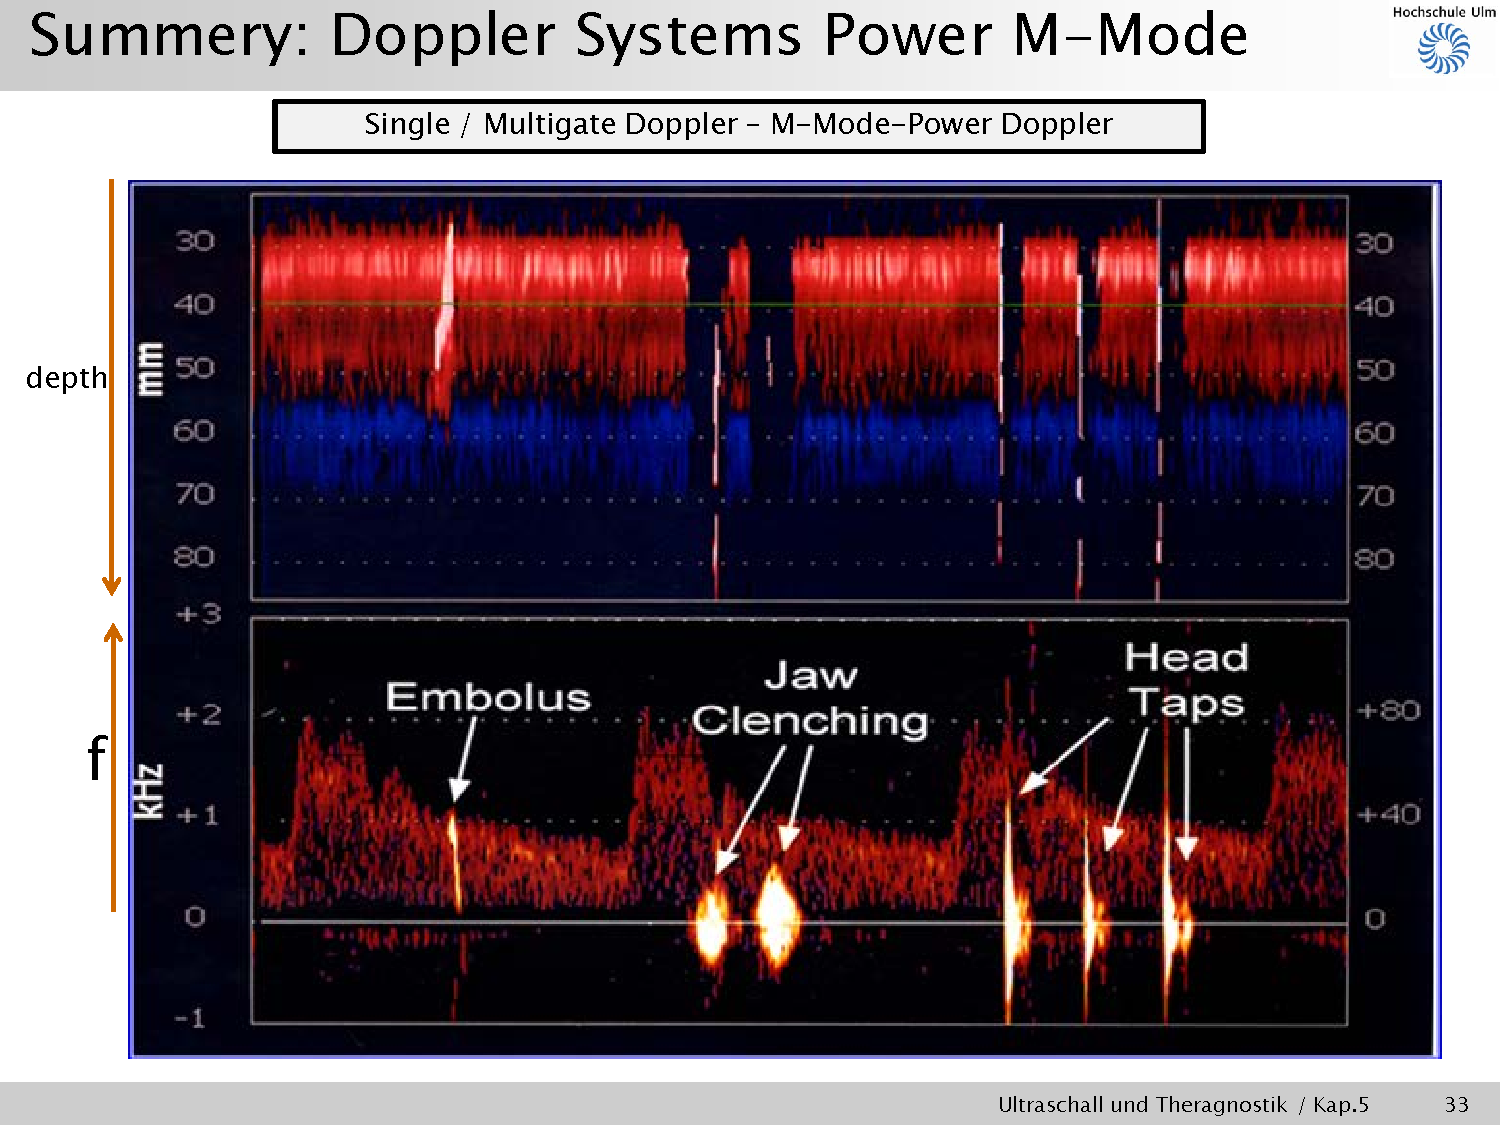
\includegraphics[trim = 2.2cm 86mm 1.3cm 3.5cm, clip=true, height=3cm, width=\textwidth]{M-Mode} 
  \caption{M-Mode}
\end{subfigure}
~
\begin{subfigure}[b]{0.48\textwidth}
  \centering
  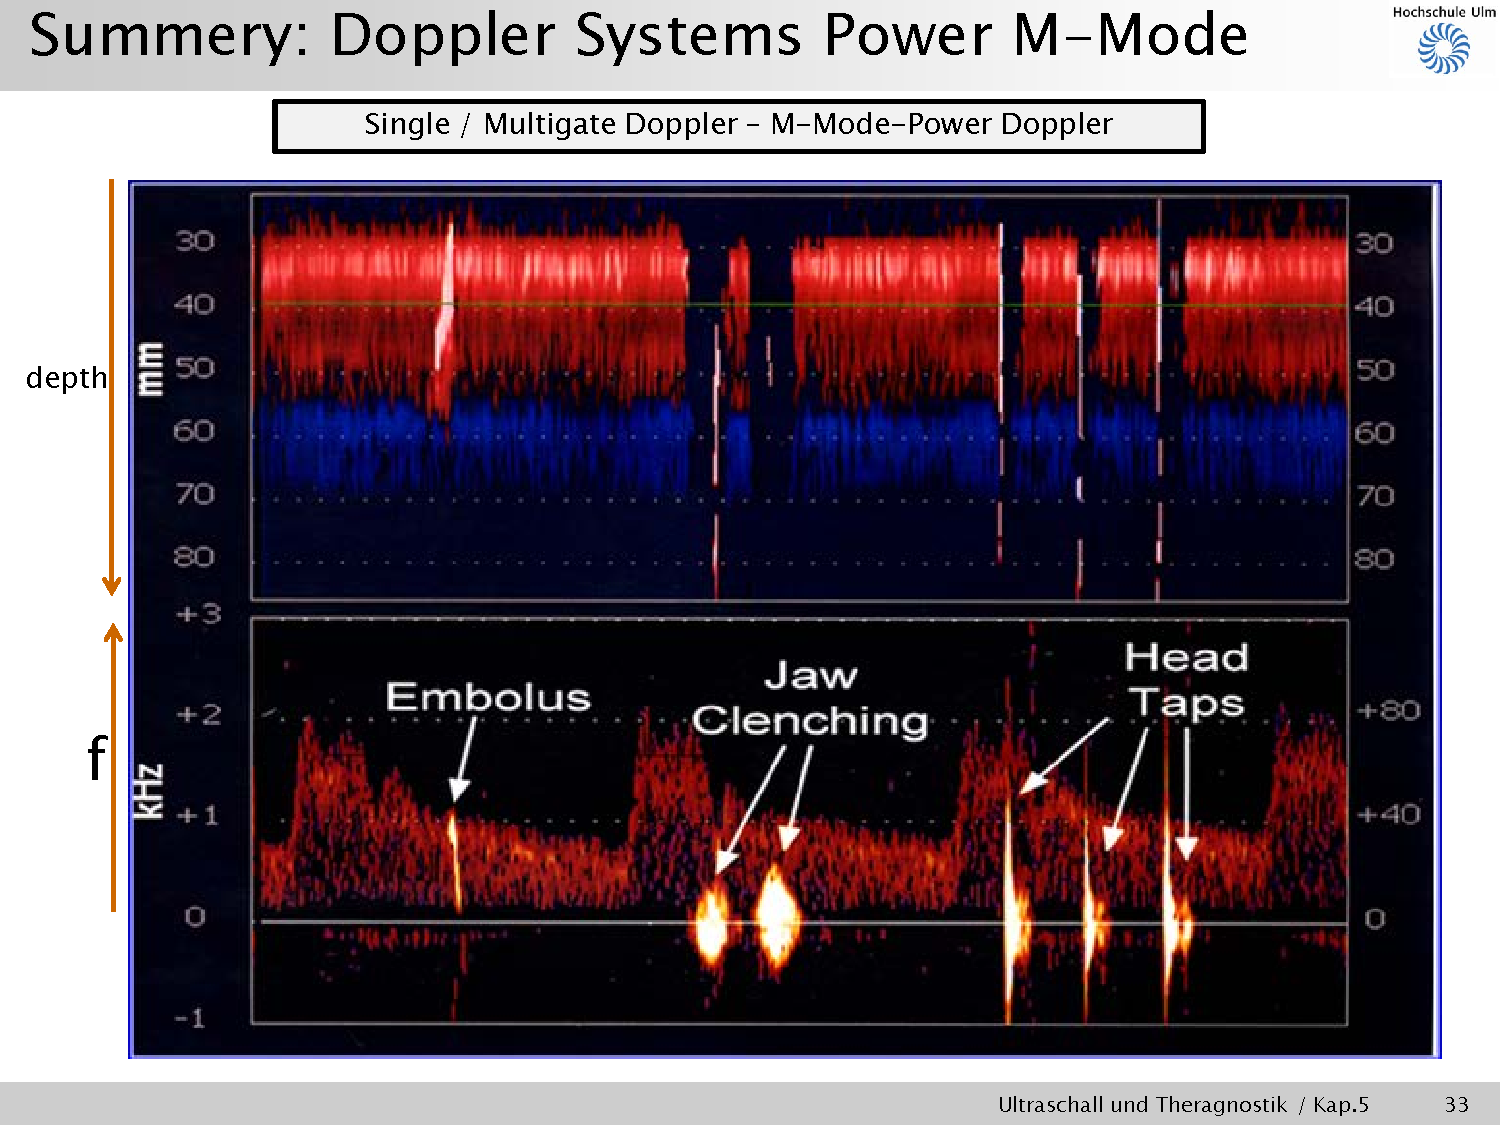
\includegraphics[trim = 2.2cm 14mm 1.3cm 10.6cm, clip=true, height=3cm, width=\textwidth]{M-Mode}  
	\caption{Doppler Spektrogram}
	\label{fig:dopp_spectrogramm}
  \label{fig:b_mode}
  \end{subfigure}
	\caption{M-Mode mit Doppler Spektrogram}
	\label{fig:m_mode}
\end{figure}

\begin{table}[h!]
\centering
\caption{Variablen des elektrischen \acs{esb} eines Piezokristalls}
\label{tab:var_esb}
\begin{tabular}{l|p{10cm}|p{3cm}}
\textbf{Variable} & \textbf{Beschreibung} & \textbf{Größenordnung} \\
\cline{1-3}
$C_0$ 	& Kapazität des Plattenkondensators mit $C_0=\varepsilon_0\cdot \varepsilon_r\cdot A/l$ & $\approx$1 nF	 \\ 
$C$ 	& Ersatzkapazität infolge der Steifigkeit des Kristalls & $\approx$0.1 pF \\
$L$		& Ersatzinduktivität infolge der Masse des Kristalls & $\approx$100 mH \\
$R$		& innere Reibung $R_i$ und Widerstand $R_{Pat}$ durch abgegebene Leistung an den Patienten $R_{Pat}=U_0^2/P_{Pat}$  & $R_i=1 \Omega$ und $R_{Pat}=50\Omega$
\end{tabular}
\end{table}